The objective of this part of the project was to create an online spatio-temporal machine learning model that could predict, using static sensors (AIRSpeck-S) and mobile sensors (AIRSpeck-P) data, the concentration levels of particulate matter in the near future (up to 6 hours). This model needs to be able to make predictions in space and time and adapt continuously in an online setting, with the expectation of being used in a real-time scenario. This model could have multiple applications such as warning system for vulnerable people, route planning, pollution monitoring and facilitate political and environmental decision making.

This project focused on making predictions of PM2.5 values given its far-reaching impact on the community and individual health conditions; however, the work described below can be applied to other PM values as well.


\section{Dataset}

The experiments performed use data that was collected by Zo\"e Petard (ZP) between June 3rd 2018 and June 26th 2018 \cite{zoe}. To simulate a real-time application of the model, two specific time periods within this dataset were chosen, given their continuity of stationary sensor readings. The first one between 3rd June 2018 to 6th June 2018, referred to as dataset A, and the second one from 23rd June 2018 to the 26th June 2018, referred to as dataset B. The datasets include continuous data from six stationary sensors and one period of mobile data collection per day, averaging $53$ minutes of mobile data per day. 

The test area is a region defined by a quadrilateral of size $0.97km$ (latitude) and $0.96km$ (longitude) in the central area of Edinburgh, totalling an area of $0.93 km^2$. This region was subdivided into a $20 \times 20$ grid, forming 400 cells of approximately $48m \times 48m$ each in size. All data was converted to these grid cells location using a Cartesian coordinate system as seen in Figure \ref{fig:grid}, using the grid cell as the resolution of the model. This level of resolution is greater than any work before ZP's spatial model \cite{zoe}.
In Figure \ref{fig:grid}, it is also possible to see the location of the stationary sensors, described in more detail in Table \ref{tab:sensors}. This table also includes information about the two mobile sensors used to collect data over several cell grids. This data is sparse both temporally, because of the duration of the collection periods and spatially, because at most one cell grid was being measured by mobile sensors at any point in time. This presented challenges to include this data in the training phase of the model created.


\begin{figure}[h] 
\centering
\includegraphics[width=0.8\linewidth]{images/mapa_com_pontos} 
\caption{Map of the test area and grid overlay. Purple cell grids indicate the locations of the stationary sensors. The coordinate system origin is marked in orange. }
\label{fig:grid}
\end{figure}

\begin{table}[h]
\centering
\resizebox{\textwidth}{!}{%
\begin{tabular}{c|ccc|ccc}
\textbf{Sensor Name} & \textbf{Sensor Identifier} & \textbf{Grid Row} & \textbf{Grid Column} & \multicolumn{3}{c}{\textbf{Calibration Factors}} \\ \cline{5-7} 
 &  &  &  & PM2.5 & Temperature & Humidity \\ \hline
Melville (MV) & 02E5F77764B873DA & 16 & 6 & 1.0 & 1.0 & 1.0 \\
Lauriston (LT) & E5FD8C55EAA37555 & 3 & 6 & 1.22 & 1.19 & 1.01 \\
Library (LY) & 200A7CED9D597407 & 8 & 5 & 1.55 & 1.51 & 1.00 \\
Tennis Court (TC) & AA0E63CF5118F98F & 13 & 13 & 2.38 & 2.31 & 0.98 \\
Bristo Square (BS) & B61241EF668DBC2C & 3 & 10 & 2.34 & 2.22 & 0.98 \\
Buccleuch Place (BP) & E786F1568F65C296 & 8 & 13 & 7.08 & 7.05 & 0.97 \\
Mobile 1 & XXM007 & - & - & 4.86 & 1.16 & 0.74 \\
Mobile 2 & XXM008 & - & - & 4.91 & 1.19 & 0.74
\end{tabular}%
}
\caption{Description of sensors and calibration factors used, with Melville sensor as reference.}
\label{tab:sensors}
\end{table}

The static sensors collected data over both datasets every 5 minutes, however, the temporal window used was 15-minute windows. This choice is justified for being not too big to allow mobile data integration, which was sampled every 10 seconds, and not too small to discern noise in the data readings. The readings were therefore re-sampled to 15 minutes using the arithmetic mean to group these values.


Figures \ref{fig:2d_mobile} and \ref{fig:hist_mobile} show the sparsity of mobile data over the grid in both datasets A and B. Almost all cell grids include less than ten readings and $45\%$ of the cells were not visited by the mobile sensor during data collection. It is possible to observe one particular grid cell with more mobile data readings because that cell is the usual location where people collecting data would start and stop using the sensor, corresponding to the Informatics Forum building. 

\begin{figure}
\centering
\begin{minipage}{.5\textwidth}
  \centering
  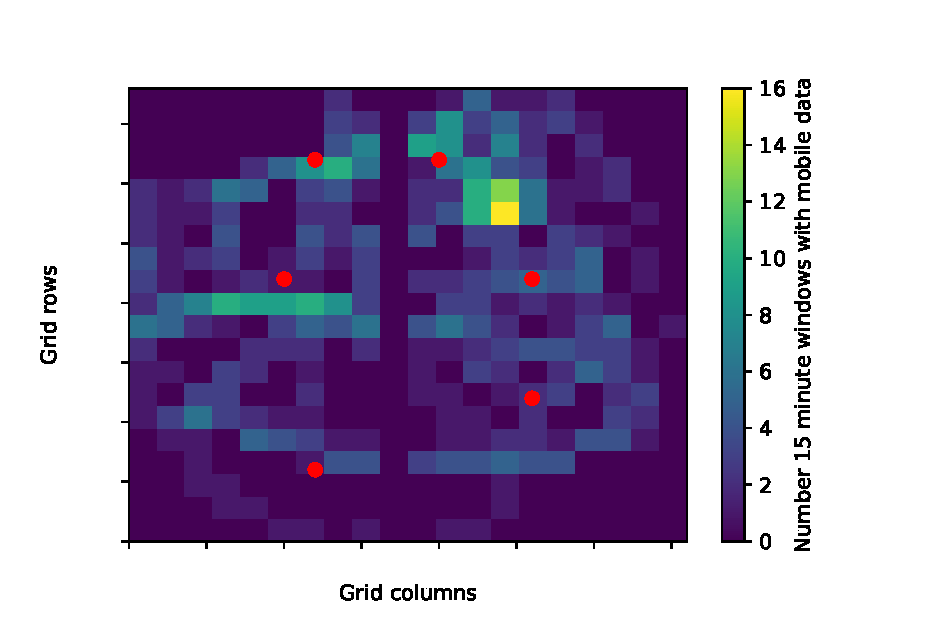
\includegraphics[width=\linewidth]{images/2D_mobile_data.eps}
  \captionsetup{width=.9\linewidth}
  \captionof{figure}{2D visualization of mobile data collected in both datasets}
  \label{fig:2d_mobile}
\end{minipage}%
\begin{minipage}{.5\textwidth}
  \centering
  \includegraphics[width=\linewidth]{images/histogram_mobile.eps}
  \captionsetup{width=.9\linewidth}
  \captionof{figure}{Histogram of grid cells by amount of mobile data collected in both datasets}
  \label{fig:hist_mobile}
\end{minipage}
\end{figure}



\subsection{Data calibration}

Similar to ZP's work, the readings of the different sensors were calibrated in reference to one of the sensors. ZP co-located the sensors in the laboratory and used the data collected during that time to calculate the factors needed for a linear scaling, presented in Table \ref{tab:sensors}. I used these factors to calibrate both stationary and mobile sensor data in both datasets.

\subsection{Outlier removal}
As another pre-processing step, outlier detection was performed on the stationary sensor data of dataset A by visual inspection (see Figure \ref{fig:raw_with_outliers}). The outliers were removed and substituted by the average of its corresponding previous and next value. Three outliers were removed by this process, and the dataset after removal can be seen in Figure \ref{fig:raw_without_outliers}. Outliers were not removed in dataset B to be able to measure the performance of the model without outlier removal, to be able to emulate a real-time use case where data was not pre-processed (other than calibration).

\begin{figure}[H] 
\centering
\vspace{1cm}
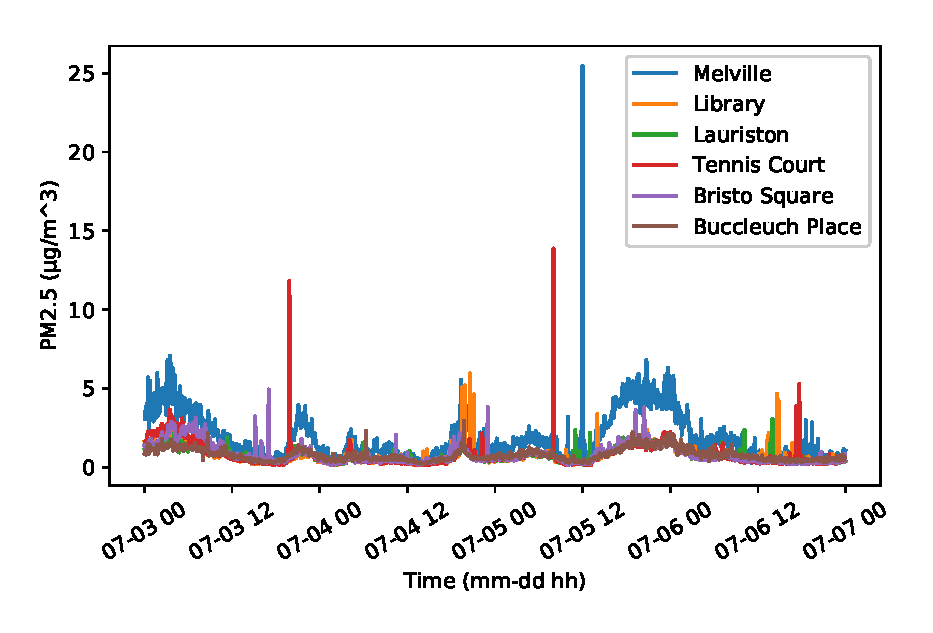
\includegraphics[width=\linewidth]{images/calibrated_data.eps} 
\caption{Calibrated readings of stationary sensors on dataset A with outliers.}
\label{fig:raw_with_outliers}
\vspace{1cm}

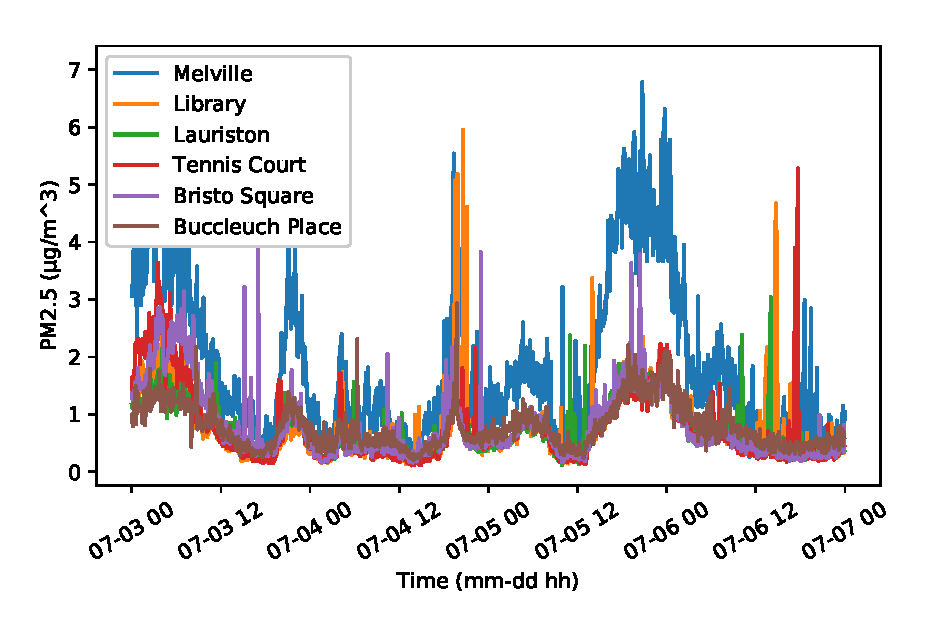
\includegraphics[width=\linewidth]{images/calibrated_data_no_outliers.eps} 
\caption{Calibrated readings of stationary sensors on dataset A without outliers.}
\label{fig:raw_without_outliers}
\vspace{1cm}

\end{figure}


\begin{table}[h]
\centering
\resizebox{\textwidth}{!}{%
\begin{tabular}{cc|cccccc|c}
\textbf{} & \textbf{Sensor} & MV & LT & LY & TC & BS & BP & \textbf{Overall} \\
\textbf{Statistical Property} & \textbf{} &  &  &  &  &  &  & \textbf{} \\ \hline
\multicolumn{2}{c|}{PM2.5 Average} & 1.83 & 0.73 & 0.75 & 0.74 & 0.80 & 0.77 & \textbf{0.94} \\
\multicolumn{2}{c|}{PM2.5 Standard Deviation} & 1.40 & 0.46 & 0.61 & 0.63 & 0.62 & 0.38 & \textbf{0.76} \\
\multicolumn{2}{c|}{PM2.5 Minimum} & 0.22 & 0.11 & 0.11 & 0.11 & 0.16 & 0.21 & \textbf{0.11} \\
\multicolumn{2}{c|}{PM2.5 Maximum} & 7.06 & 3.05 & 5.95 & 5.28 & 4.93 & 2.93 & \textbf{7.06} \\ \hline
\multicolumn{2}{c|}{Temperature average} & 18.89 & 12.28 & 9.21 & 6.6 & 6.95 & 2.43 & \textbf{9.39} \\
\multicolumn{2}{c|}{Temperature Standard Deviation} & 4.38 & 2.65 & 2.06 & 1.64 & 1.58 & 0.53 & \textbf{2.45} \\ \hline
\multicolumn{2}{c|}{Humidity Average} & 63.53 & 37.93 & 32.45 & 21.23 & 22.26 & 7.27 & \textbf{30.78} \\
\multicolumn{2}{c|}{Humidity Standard Deviation} & 13.98 & 8.14 & 6.61 & 5.18 & 4.99 & 1.54 & \textbf{7.74}
\end{tabular}%
}
\caption{Statistical properties of the calibrated static data of dataset A}
\label{tab:statisticsA}
\end{table}

\begin{table}[h]
\centering
\resizebox{\textwidth}{!}{%
\begin{tabular}{cc|cccccc|c}
\textbf{} & \textbf{Sensor} & MV & LT & LY & TC & BS & BP & \textbf{Overall} \\
\textbf{Statistical Property} & \textbf{} &  &  &  &  &  &  & \textbf{} \\ \hline
\multicolumn{2}{c|}{PM2.5 Average} & 1.09 & 0.44 & 0.45 & 0.50 & 0.51 & 0.53 & \textbf{0.59} \\
\multicolumn{2}{c|}{PM2.5 Standard Deviation} & 3.59 & 1.29 & 0.61 & 1.05 & 0.85 & 0.28 & \textbf{1.67} \\
\multicolumn{2}{c|}{PM2.5 Minimum} & 0.11 & 0.08 & 0.07 & 0.06 & 0.09 & 0.00 & \textbf{0.00} \\
\multicolumn{2}{c|}{PM2.5 Maximum} & 118.84 & 43.03 & 9.35 & 28.08 & 24.69 & 4.35 & \textbf{118.84} \\ \hline
\multicolumn{2}{c|}{Temperature average} & 21.36 & 13.68 & 10.08 & 7.02 & 7.66 & 2.55 & \textbf{10.38} \\
\multicolumn{2}{c|}{Temperature Standard Deviation} & 5.12 & 2.99 & 2.18 & 1.68 & 1.72 & 0.52 & \textbf{2.77} \\ \hline
\multicolumn{2}{c|}{Humidity Average} & 59.72 & 36.54 & 31.88 & 21.34 & 21.57 & 7.47 & \textbf{29,75} \\
\multicolumn{2}{c|}{Humidity Standard Deviation} & 16.82 & 9.96 & 8.01 & 5.99 & 5.84 & 1.97 & \textbf{9.31}
\end{tabular}%
}
\caption{Statistical properties of the calibrated static data of dataset B}
\label{tab:statisticsB}
\end{table}


\section{Model selection}
The online spatio-temporal model can be divided into two main components: the temporal model and the spatial model. The choice of the model used in each of these components was based on the work performed by Ivan Angelinin and Mantas Miksys, which concluded that from the models analysed, the best performing temporal model was the Passive-Aggressive Regressor \cite{ivan}, and the best performing spatial model was Ordinary Kriging and Radial Basis Functions \cite{mantas}. Citing Angelinin, "Kriging has the best results in most papers and is widely used approach that has been shown to work well in many different domains"\cite{ivan}. This was verified by the literature survey performed \cite{st_state} \cite{env_book}.

\section{Online Temporal model: Passive-Aggressive Regressor}
\label{chap:par}
The Passive-Aggressive Regressor (PAR) model was first introduced by Crammer \textit{et al.} and is a margin-based online machine learning model that can be used for classification, regression, uni-class prediction and sequence prediction \cite{crammer}. Given its online characteristics, it has the ability to receive training data in a streaming setting.
Predictions are performed with a linear model, and the linear parameters are updated when new data points are fed to the model. The parameter updates can be either passive, that is, neglected, when the error is small, and aggressive when the error is significant, giving the model the passive/aggressive duality. This error threshold that defines the boundary of aggressiveness  is determined with a hyperparameter, referred to as epsilon ($\varepsilon$), at model instantiation. It is also possible to regulate the magnitude of aggressiveness of the algorithm, using a hyperparameter referred to as C, the maximum step size. This project used the PAR implementation available on scikit-learn, a machine learning package for python \cite{scikit-learn}.

\section{Spatial model: Ordinary Kriging}
\label{chap:ok}
Kriging is a family of geostatistic methods that estimates a variable in locations where data is not available, using nearby observations of that variable or irregular spaced data points. Several members of that family include Simple Kriging, Ordinary Kriging, Universal Kriging and Regression Kriging. These variants differ in the way that weight parameters are calculated for the interpolation. It is widely used in environmental sciences \cite{envscience}, hydrology \cite{hydrology}, mining \cite{mining} and other geostatistical applications. In this case, it will be used as a spatial interpolation technique to estimate PM values in grid cells where observations with sensors did not occur, filling the data that was sparsely collected.

Ordinary Kriging is one of the most popular Kriging techniques and is described as "best linear unbiased estimator". "Best" is derived from aiming to minimise the variance of errors, "linear" because it is a weighted linear combination of available data and "unbiased" because it tries to have residual or error equal to zero \cite{ordkriging}.
The implementation of Ordinary Kriging used in this project was PyKrige \cite{pykrige} by Benjamin Murphy.

In terms of performance for a real-time application, there were not any significant computational costs during the experiments performed, but this may be due to the area being used of approximately $1 km^2$. The current implementation did not reach a computational cost for the need to improve implementation efficiency, but in a real-time application with a much bigger area, it may reach a point that may need more computational power or a more efficient approach to Kriging, as the time complexity of Ordinary Kriging is $O(N^4)$ where N is the number of interpolated points \cite{efficientkriging}. More efficient solutions have been proposed and demonstrated to be faster, with time complexity $O(N^3)$ and using iterative solvers \cite{efficientkriging}, which could allow even bigger test areas.

\section{Online Spatio-temporal model: proposed model}

The proposed model combines the passive-aggressive regressor and ordinary kriging to allow for an online spatio-temporal model, capable of making predictions for all the grids of the test area. The most significant advantage of this model is that it uses the mobile data collected in addition to the static sensors and although this data may be sparse in both time and space, it is essential to improve the performance of the predictions.

Based on the two models described in section \ref{chap:par} and \ref{chap:ok}, the proposed model works as follows: In every time step, the data gathered in each grid cell is averaged. This produces a PM2.5 value for each cell grid where data was collected. The cells where data was not collected are then filled with values with Ordinary Kriging. In every time step, the model produces a grid filled with values read or originating from Ordinary Kriging. 

A Passive-Aggressive Regressor is instantiated for each of the grid cells in the test area, and each of the PAR models is fed the corresponding value coming from the grid computed at each time cell. That 2D grid of PAR models is then available to produce predictions for future time steps. This sequence can be observed in Figure \ref{fig:model_diagram}.

After the predictions are output by that model, it is corrected using the past errors made either on the same cell, neighbouring cells or globally. The error made in every prediction is also stored to adjust for future projections, as seen in Figure \ref{fig:error_diagram}. 

Several methods of error correction can be applied to discount the bias present in the model output prediction such as the last value seen, mean, median, and the diverse spectrum of regression models. The history of errors contribute to the future error correction because a tendency of errors is captured and prevented the best way possible in every prediction. The more errors are recorded in each grid cell, the more information we have to compute these metrics and more robust they tend to become to improve predictions. In Section \ref{improvement}
, several of these methods are tested and evaluated with the data available.


\begin{figure}[H] 
\centering
\vspace{1cm}
\includegraphics[width=\linewidth]{images/model_diagram.png} 
\caption{Online spatio-temporal model diagram. "X" denotes the cells where data was collected either with stationary or mobile sensors. "o" denotes the values interpolated from the cells with "X".}
\label{fig:model_diagram}
\vspace{1cm}
\end{figure}

\begin{figure}[H]
\centering
\includegraphics[width=\linewidth]{images/error_correction_diagram.png} 
\caption{Error correction algorithm diagram}
\label{fig:error_diagram}
\end{figure}

The error calculation is detailed in Figure \ref{fig:delta_correction}. The error is the difference between the prediction made in the past and the ground truth seen at the time corresponding to the prediction goal.  That error is stored in a data structure for correction of future predictions, along with the location and time of the occurrence.

\begin{figure}[H]
\centering
\includegraphics[width=\linewidth]{images/delta_correction.png} 
\caption{Error computation and storage diagram}
\label{fig:delta_correction}
\vspace{1cm}
\end{figure}


\section{Performance metrics}
The model was evaluated using several metrics on different test sets, depending on the experiment. The ground truth values used were the values read in the timestep that the prediction aimed for in the future. Therefore, only cell grids with values read in the future (after the simulated present of the model) can be used to measure the performance of the model.
Consider $O$ the observed value collected by the sensors and $P$ the predicted value (output of the model). Also, consider error $E$ as the difference between the ground truth and the predicted value ( $E = O-P$ ). The absolute error $AE$ is, therefore, the absolute value of the error ($AE = \mid O-P \mid$).
Mean Absolute Error (MAE) was the most used metric used to evaluate the performance of the model. Mean Absolute Error, described as the average of the Absolute Errors, has the same unit as the original data and can be simply defined by:

\[MAE = \frac{\sum_{i=1}^{n} AE_i}{n} = \frac{\sum_{i=1}^{n} \mid E_i \mid}{n} = \frac{\sum_{i=1}^{n} \mid O_i-P_i \mid}{n}\]

MAE ranges from 0 to $\infty$ and the lower the value, the better the model being evaluated.

Root Squared Error (RSE) is a similar metric that gives more weight to higher errors because these are squared. The same amount of absolute error divided over several observations and predictions would yield a lower RSE than the same absolute error observed in a single observations and prediction. RSE is similarly defined by: 

\[RSE = \frac{\sum_{i=1}^{n} E_i^2}{n} = \frac{\sum_{i=1}^{n} (O_i-P_i)^2}{n}\]

The lower the RSE, the better the model performance is. Lastly, Root Mean Square Deviation (RMSE), also referred to as Root Mean Square Error (RMSE) is the square root of RSE, therefore behaves similarly to it. The lower the RMSE, the better the performance.


\section{Baselines}
\label{chap:baselines}

Two types of baselines were used to compare and evaluate the predictions: one purely on the temporal basis and another one on the spatio-temporal basis.
The temporal baseline can only be applied in the cell grids with stationary sensors as these are the only ones that have continuous data in the temporal dimension.
Comparable work performed by Ivan Angelinin and Mantas Miksys used the value read 24 hours before and an RMSD of 5 respectively as the temporal baseline.
However, in addition to these benchmarks, two new baselines were developed, which performed better than the previous ones. The new baselines correspond to using the past 60 minutes or the last 15 minutes to predict the value. These are predictions that include more recent data observed, and because the data is temporally closer to what is trying to be predicted, better results were expected. Table \ref{tab:tempbaselines} shows the results of the temporal baseline applied to dataset A.

\begin{table}[h]
\centering
\begin{tabular}{c|ccc}
\textbf{} & \textbf{\begin{tabular}[c]{@{}c@{}}Mean Absolute \\ Error\end{tabular}} & \textbf{\begin{tabular}[c]{@{}c@{}}Mean Squared\\ Error\end{tabular}} & \textbf{\begin{tabular}[c]{@{}c@{}}Root Mean \\ Square Deviation\end{tabular}} \\ \hline
Ivan Angelinin's Baseline & 0.65 & 1.01 & 1.00 \\ \hline
Mantas Miksys' Baseline & - & - & 5 \\ \hline
60 minute Basline & 0.25 & 0.15 & 0.39 \\ \hline
\textbf{\begin{tabular}[c]{@{}c@{}}15 minute  Baseline\\ (proposed baseline)\end{tabular}} & 0.16 & 0.08 & 0.28 \\ \hline
\end{tabular}
\caption{Temporal Baselines Results}
\label{tab:tempbaselines}
\end{table}

The second type of baseline used is a spatio-temporal baseline. The best baseline found consists of predicting the PM2.5 concentration level in a cell grid at a specific timestep by using the most recent value read in the closest stationary sensor available. This baseline yielded the following results for dataset A:
\begin{itemize}
  \item Mean Absolute Error: 2.81
  \item Root Mean Squared Error: 3.87
\end{itemize}
The model outperformed the baseline model regardless whether or not error correction was used (see \autoref{chap:st_results}).

